\documentclass{article}
\usepackage{graphicx}
\usepackage{amsmath}
\usepackage{booktabs}
\usepackage{caption}
\usepackage{hyperref}
\usepackage[a4paper, margin=1in]{geometry}
\usepackage{listings}
\usepackage{float}

\lstset{
    basicstyle=\ttfamily\small,
    breaklines=true,
    frame=single
}

\title{Technical Report on Data Processing and Machine Learning for Crack Detection in Glass Fiber Composites}
\author{A. Uğurveren}
\date{\today}

\begin{document}

\maketitle

\section{Data Acquisition and Preprocessing}

The data for this project originates from two main sources: the FBG interrogator, which provides wavelength data from the sensors in `.txt` files, and the three-point bending test machine, which records mechanical data such as force and displacement, stored in a structured `.xlsx` file.

\subsection{Key Data Resources}
For a more detailed understanding of the raw data, several key files are available in the Teams Channel:
\begin{itemize}
    \item \texttt{wavelengths\_by\_file.png}: This image provides a plot of wavelength versus time for each test sequence recorded by the FBG interrogator. It is useful for visualizing the raw sensor output over the course of the experiments. I would recommend to download it before examining because Teams app sometimes is not capable to show.
    \item \texttt{manual\_data.xlsx}: This Excel file contains the data recorded manually from the three-point bending machine, including force, displacement, and crack detection data.
    \item \texttt{merged\_experimental\_data}: This directory contains the merged data from the FBG interrogator and the bending machine for each test sequence. The CSV files are named with a convention that includes span length, layer count, and test number. An 's' suffix after the test number (e.g., \texttt{-s}) indicates a smaller sample type with a different Young's Modulus. An example filename is: \texttt{merged\_11cm-12layers-1-s\_20250915\_1440.csv}.
    \item \texttt{interrogator\_data}: This directory holds the raw interrogator data as `.txt` files for each sequence. The naming convention is consistent with the merged data, including the 's' identifier for small samples.
\end{itemize}

\subsection{Data Merging and Segmentation}
The first step is to merge and synchronize these two data sources. This process is handled by a series of automated scripts.

\subsubsection{Automated Batch Processing}
An automated script handles the merging process for a whole directory of interrogator data files. For each file, it intelligently determines the corresponding sheet in the mechanical test data `.xlsx` file. A key feature of this process is its robustness: it performs a parameter sweep to find the optimal settings for peak detection for each individual experiment file. This ensures the highest quality data is extracted from each test run. The script generates a timestamped output directory for each run, containing the merged `.csv` files.

\subsubsection{Signal Smoothing and Segmentation}
The raw wavelength signal, which can be noisy, is first smoothed using a median filter. The script then needs to identify the distinct segments in the data that correspond to the repeated applications of force. This is a critical step and is accomplished using peak detection on a representative signal.

The \texttt{scipy.signal.find\_peaks} function is used for this purpose, with parameters like \texttt{peak\_height}, \texttt{peak\_distance}, and \texttt{peak\_prominence} being tuned by the batch script to accurately isolate the experimental repetitions.

\subsubsection{Mechanical Test Data}
The mechanical test data, containing parameters like the force applied and the resulting displacement, is stored in a structured format. This information is crucial as it provides the ground truth for the physical state of the material during the experiments. A sample of this data is shown in Table \ref{tab:metadata_sample}.

\begin{table}[h!]
\centering
\begin{tabular}{@{}llll@{}}
\toprule
Air Pressure (bar) & Force (N) & Displacement (mm) & Crack \\ \midrule
1.0 & 147 & 36.37 & 0 \\
1.2 & 163 & 36.55 & 0 \\
1.4 & 180 & 36.85 & 0 \\
1.6 & 197 & 37.10 & 0 \\
1.8 & 214 & 37.40 & 0 \\ \bottomrule
\end{tabular}
\caption{Sample of Mechanical Test Data}
\label{tab:metadata_sample}
\end{table}

\subsubsection{Sample of Merged Data}
The result of this preprocessing is a set of `.csv` files, one for each experiment, containing the synchronized mechanical and sensor data. Table \ref{tab:sample_data} shows an expanded view with 20 rows from a sample file, focusing on the data from the FBG channel.

\begin{table}[h!]
\centering
\resizebox{\textwidth}{!}{%
\begin{tabular}{@{}lllllllll@{}}
\toprule
Air Pressure (bar) & Force (N) & Disp. (mm) & Seg Start & Seg End & Timestamp & WL\_ch2 & WL\_ch2\_std & Crack \\ \midrule
1.0 & 147 & 36.37 & 197 & 226 & 2025-08-11 14:03:58 & 1539.534 & 0.3118 & 0 \\
1.0 & 147 & 36.37 & 297 & 332 & 2025-08-11 14:04:09 & 1539.528 & 0.2796 & 0 \\
1.0 & 147 & 36.37 & 399 & 433 & 2025-08-11 14:04:19 & 1539.533 & 0.2567 & 0 \\
1.0 & 147 & 36.37 & 508 & 543 & 2025-08-11 14:04:30 & 1539.524 & 0.2879 & 0 \\
1.0 & 147 & 36.37 & 641 & 673 & 2025-08-11 14:04:44 & 1539.504 & 0.2830 & 0 \\
1.0 & 147 & 36.37 & 729 & 760 & 2025-08-11 14:04:54 & 1539.517 & 0.2669 & 0 \\
1.0 & 147 & 36.37 & 821 & 853 & 2025-08-11 14:05:04 & 1539.537 & 0.2693 & 0 \\
1.0 & 147 & 36.37 & 917 & 952 & 2025-08-11 14:05:14 & 1539.515 & 0.2797 & 0 \\
1.0 & 147 & 36.37 & 1028 & 1062 & 2025-08-11 14:05:25 & 1539.518 & 0.2530 & 0 \\
1.0 & 147 & 36.37 & 1126 & 1154 & 2025-08-11 14:05:36 & 1539.507 & 0.2834 & 0 \\
1.2 & 163 & 36.55 & 1415 & 1449 & 2025-08-11 14:06:07 & 1539.667 & 0.3271 & 0 \\
1.2 & 163 & 36.55 & 1513 & 1544 & 2025-08-11 14:06:17 & 1539.660 & 0.3041 & 0 \\
1.2 & 163 & 36.55 & 1611 & 1643 & 2025-08-11 14:06:28 & 1539.649 & 0.3189 & 0 \\
1.2 & 163 & 36.55 & 1695 & 1729 & 2025-08-11 14:06:37 & 1539.668 & 0.3216 & 0 \\
1.2 & 163 & 36.55 & 1784 & 1814 & 2025-08-11 14:06:47 & 1539.688 & 0.3465 & 0 \\
1.2 & 163 & 36.55 & 1880 & 1914 & 2025-08-11 14:06:57 & 1539.673 & 0.3105 & 0 \\
1.2 & 163 & 36.55 & 1977 & 2012 & 2025-08-11 14:07:07 & 1539.664 & 0.3111 & 0 \\
1.2 & 163 & 36.55 & 2084 & 2115 & 2025-08-11 14:07:18 & 1539.642 & 0.3645 & 0 \\
1.2 & 163 & 36.55 & 2170 & 2200 & 2025-08-11 14:07:28 & 1539.688 & 0.3144 & 0 \\
1.2 & 163 & 36.55 & 2262 & 2295 & 2025-08-11 14:07:38 & 1539.684 & 0.3193 & 0 \\
\bottomrule
\end{tabular}%
}
\caption{Detailed sample rows from a merged data file}
\label{tab:sample_data}
\end{table}

\subsection{Feature Engineering and Selection}
Once the data is merged, the next step is to engineer features that will be fed into the machine learning models.

Based on domain knowledge and the available data, a set of 9 features was engineered:
\begin{table}[h!]
\centering
\begin{tabular}{@{}ll@{}}
\toprule
Feature Name & Description \\ \midrule
\texttt{WL\_ch2} & The absolute wavelength from the central Bragg channel. \\
\texttt{WL\_ch2\_std} & The standard deviation of the wavelength in a segment. \\
\texttt{delta\_wl\_ch2} & Change in wavelength relative to the start of the measurement. \\
\texttt{Force (N)} & The force applied by the bending machine. \\
\texttt{Displacement (mm)} & The displacement of the composite beam. \\
\texttt{Air Pressure (bar)} & The air pressure applied during the test. \\
\texttt{delta\_wl\_rate} & The rate of change of the delta wavelength. \\
\texttt{delta\_disp\_rate} & The rate of change of the displacement. \\
\texttt{is\_small\_sample} & A binary feature indicating the sample type. \\ \bottomrule
\end{tabular}
\caption{Engineered Features for Machine Learning Models}
\label{tab:features}
\end{table}

The central Bragg channel (\texttt{WL\_ch2}) was chosen as it consistently provided the most stable and representative signal for strain measurement across the experiments. The "rate" features are particularly important as they help the model understand the dynamics of the material's response to stress.

\section{Model Exploration with PyCaret}

To establish a performance baseline and explore a wide variety of standard machine learning models, the PyCaret library was employed. Its \texttt{compare\_models()} function was used to train and evaluate multiple classifiers on the engineered feature set.

The results from this analysis showed that tree-based ensemble models, specifically Random Forest, performed exceptionally well. This provided a strong indication that the engineered features were highly informative and that a powerful classification model could be built for this task. The best model from this process was saved for later comparison.

\section{Neural Network Implementation}
While the initial exploration provided excellent results with classical models, deep learning models were also implemented to capture potentially more complex temporal patterns in the data. The entire pipeline, from data loading to training and evaluation, was integrated into a unified workflow.

\subsection{Sequence Generation}
To prepare the data for time-series models (like CNNs), the individual data points are grouped by experimental runs (based on air pressure) and then transformed into sequences of a fixed length using a sliding window approach. A sequence length of 50 time steps was used. The label for each sequence is determined by the crack state 5 time steps ahead of the sequence (a prediction horizon of 5), making the model predictive in nature.

\subsection{Data Normalization}
Before training, all features were normalized using \texttt{StandardScaler} from scikit-learn. Crucially, the scaler was fitted \textbf{only} on the training dataset to prevent any information leakage from the validation or test sets into the training process. This same fitted scaler was then used to transform the validation and test sets.

\subsection{Model Architectures}
Several models were implemented and compared:
\begin{itemize}
    \item \textbf{Random Forest, KNN, Gaussian Naive Bayes:} These classical models from scikit-learn were used as strong baselines.
    \item \textbf{CNN Model:} A Convolutional Neural Network was implemented in PyTorch. The architecture consists of three 1D convolutional layers with ReLU activation, followed by a global average pooling layer and a final fully connected layer for classification. The number of filters in the convolutional layers increases from 32 to 64 to 128, allowing the model to learn increasingly complex features. Dropout with p=0.2 was used to prevent overfitting.
\end{itemize}

\subsection{Training and Evaluation}
The neural network models were trained using the Adam optimizer and a Cross-Entropy Loss function. To counter the imbalanced nature of the dataset (many more "No Crack" samples than "Crack" samples), class weights were calculated and applied to the loss function. This gives more importance to the minority classes during training.

An early stopping mechanism was used with a patience of 10 epochs. The model's state was saved whenever the validation loss improved, ensuring that the best performing model on the validation set was retained.

\section{Results}
The performance of all models was evaluated on the held-out test set. The primary metric for evaluation was the confusion matrix, which visualizes the performance of the classification algorithm.

\begin{figure}[H]
    \centering
    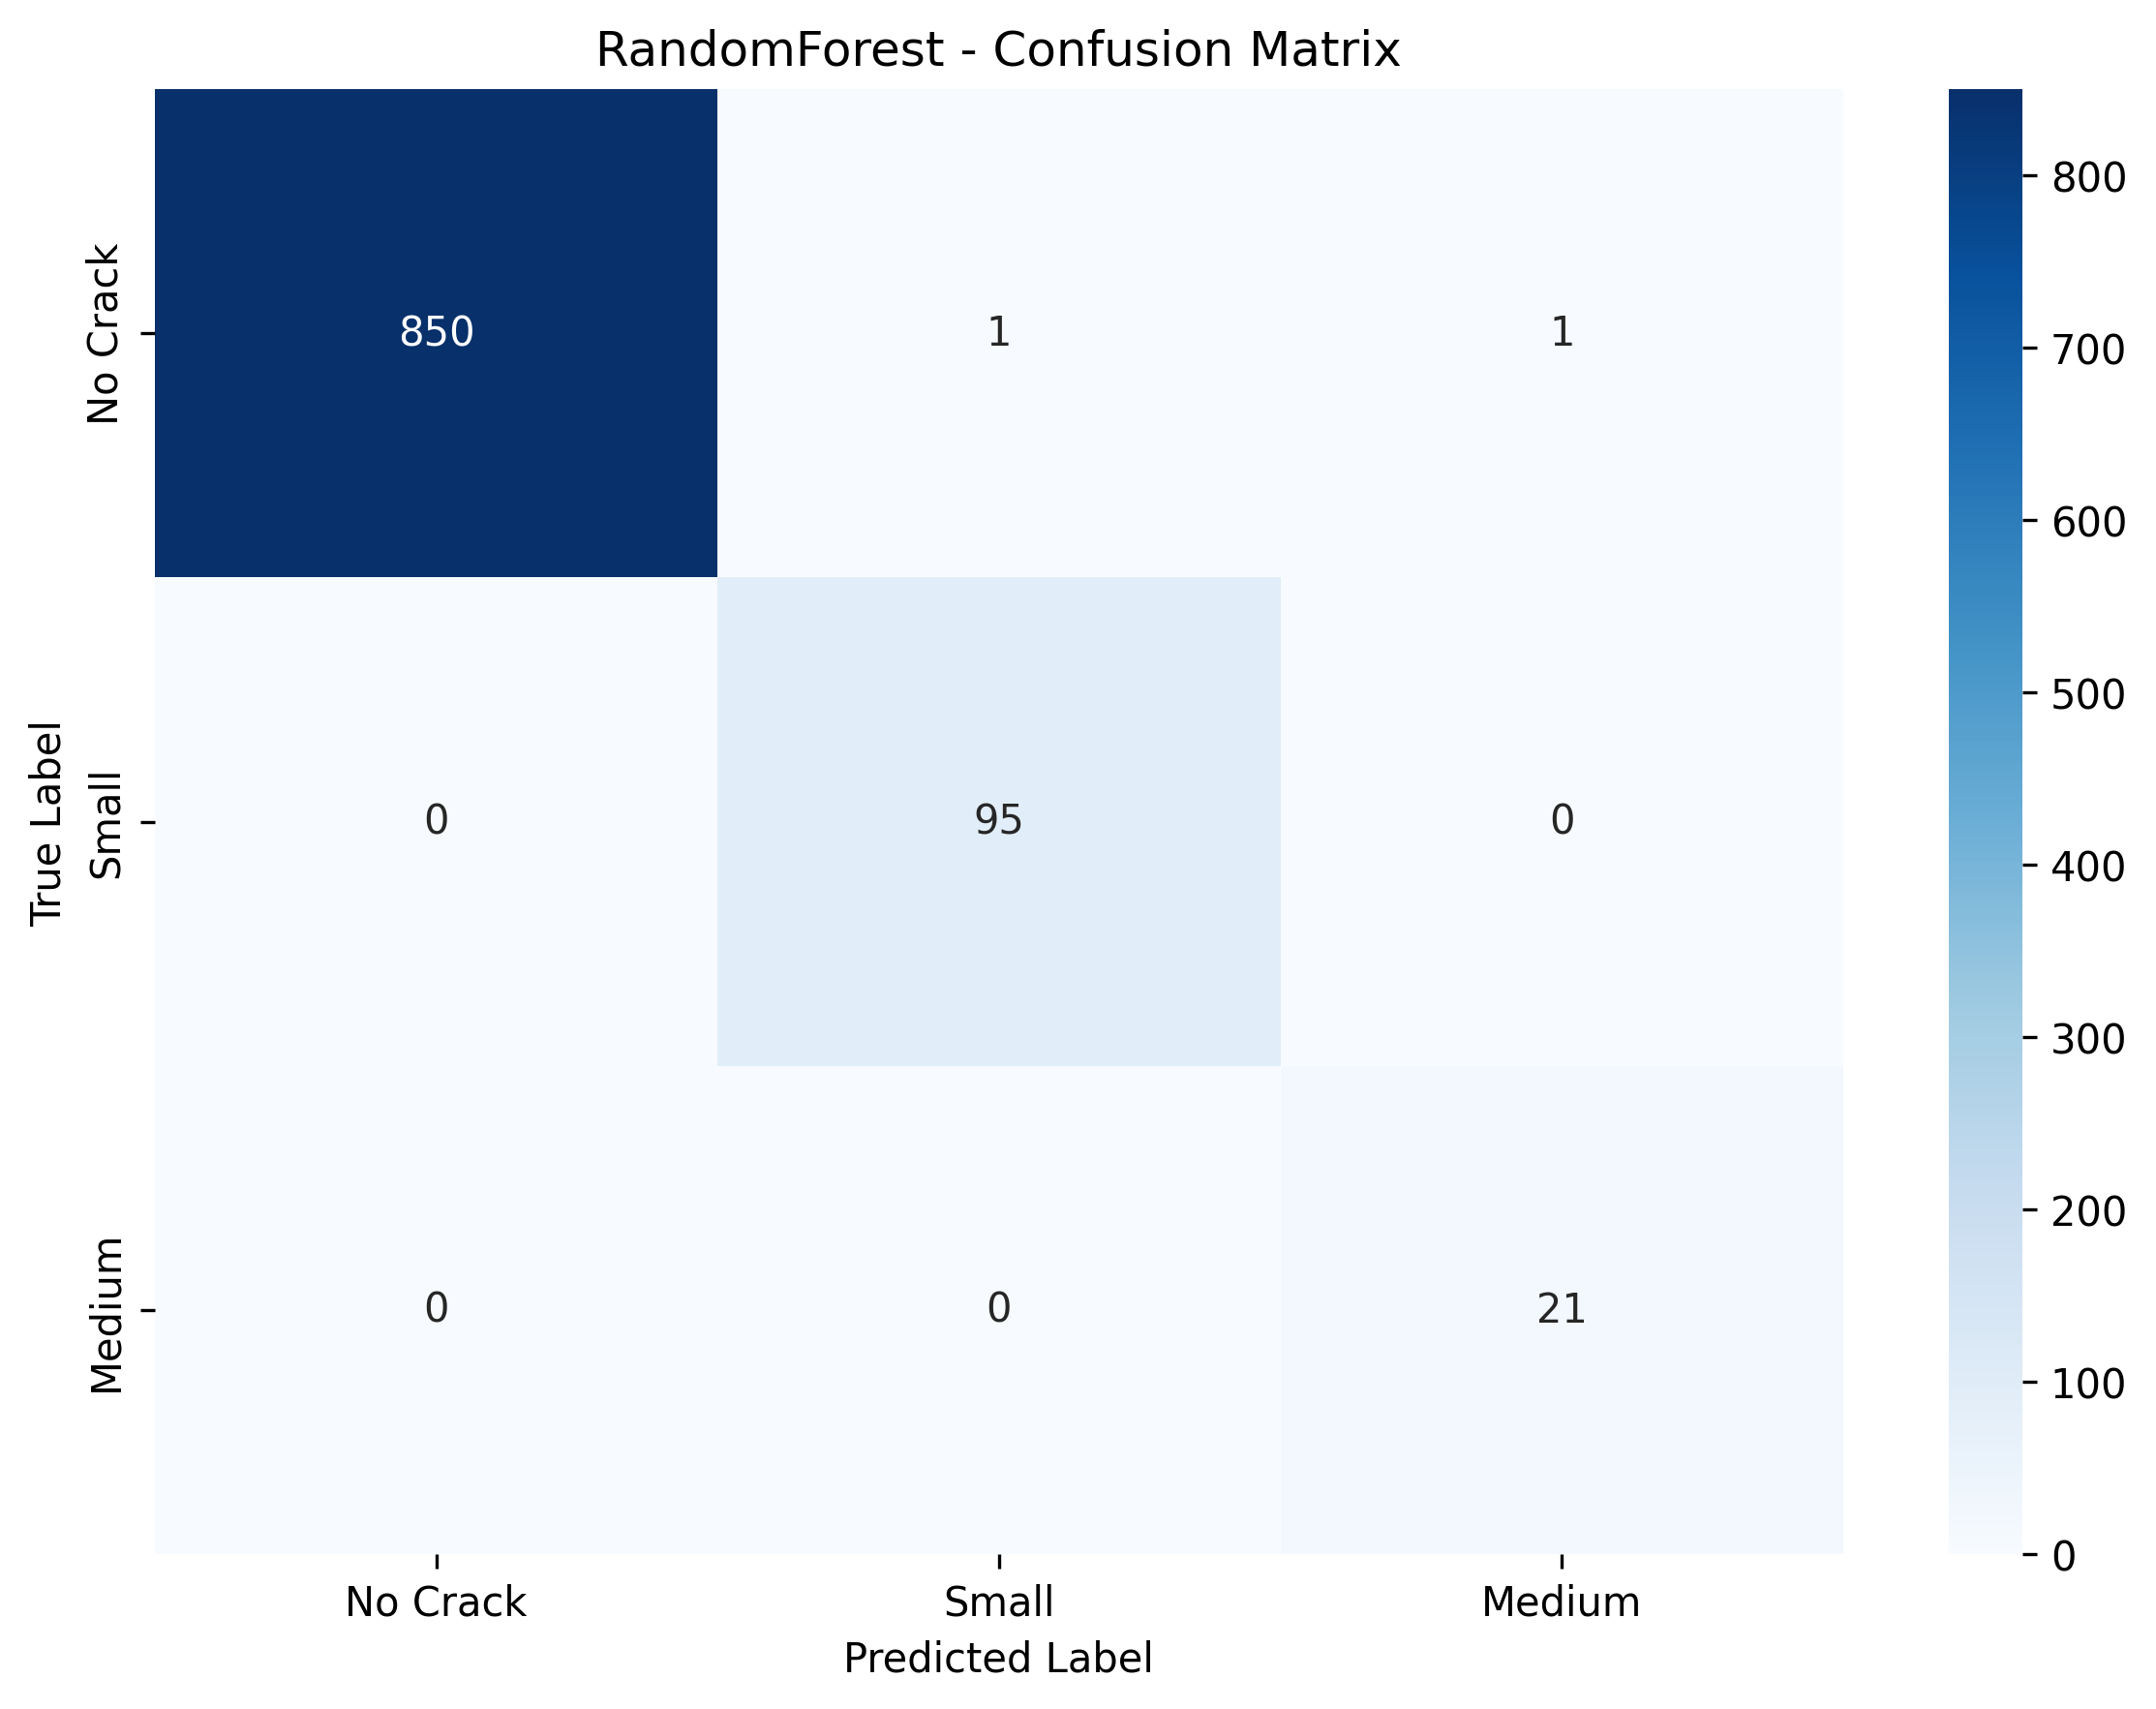
\includegraphics[width=0.7\textwidth]{img/RandomForest_confusion_matrix_100pct.png}
    \caption{Confusion Matrix for the Random Forest Model.}
    \label{fig:rf_cm}
\end{figure}

\begin{figure}[H]
    \centering
    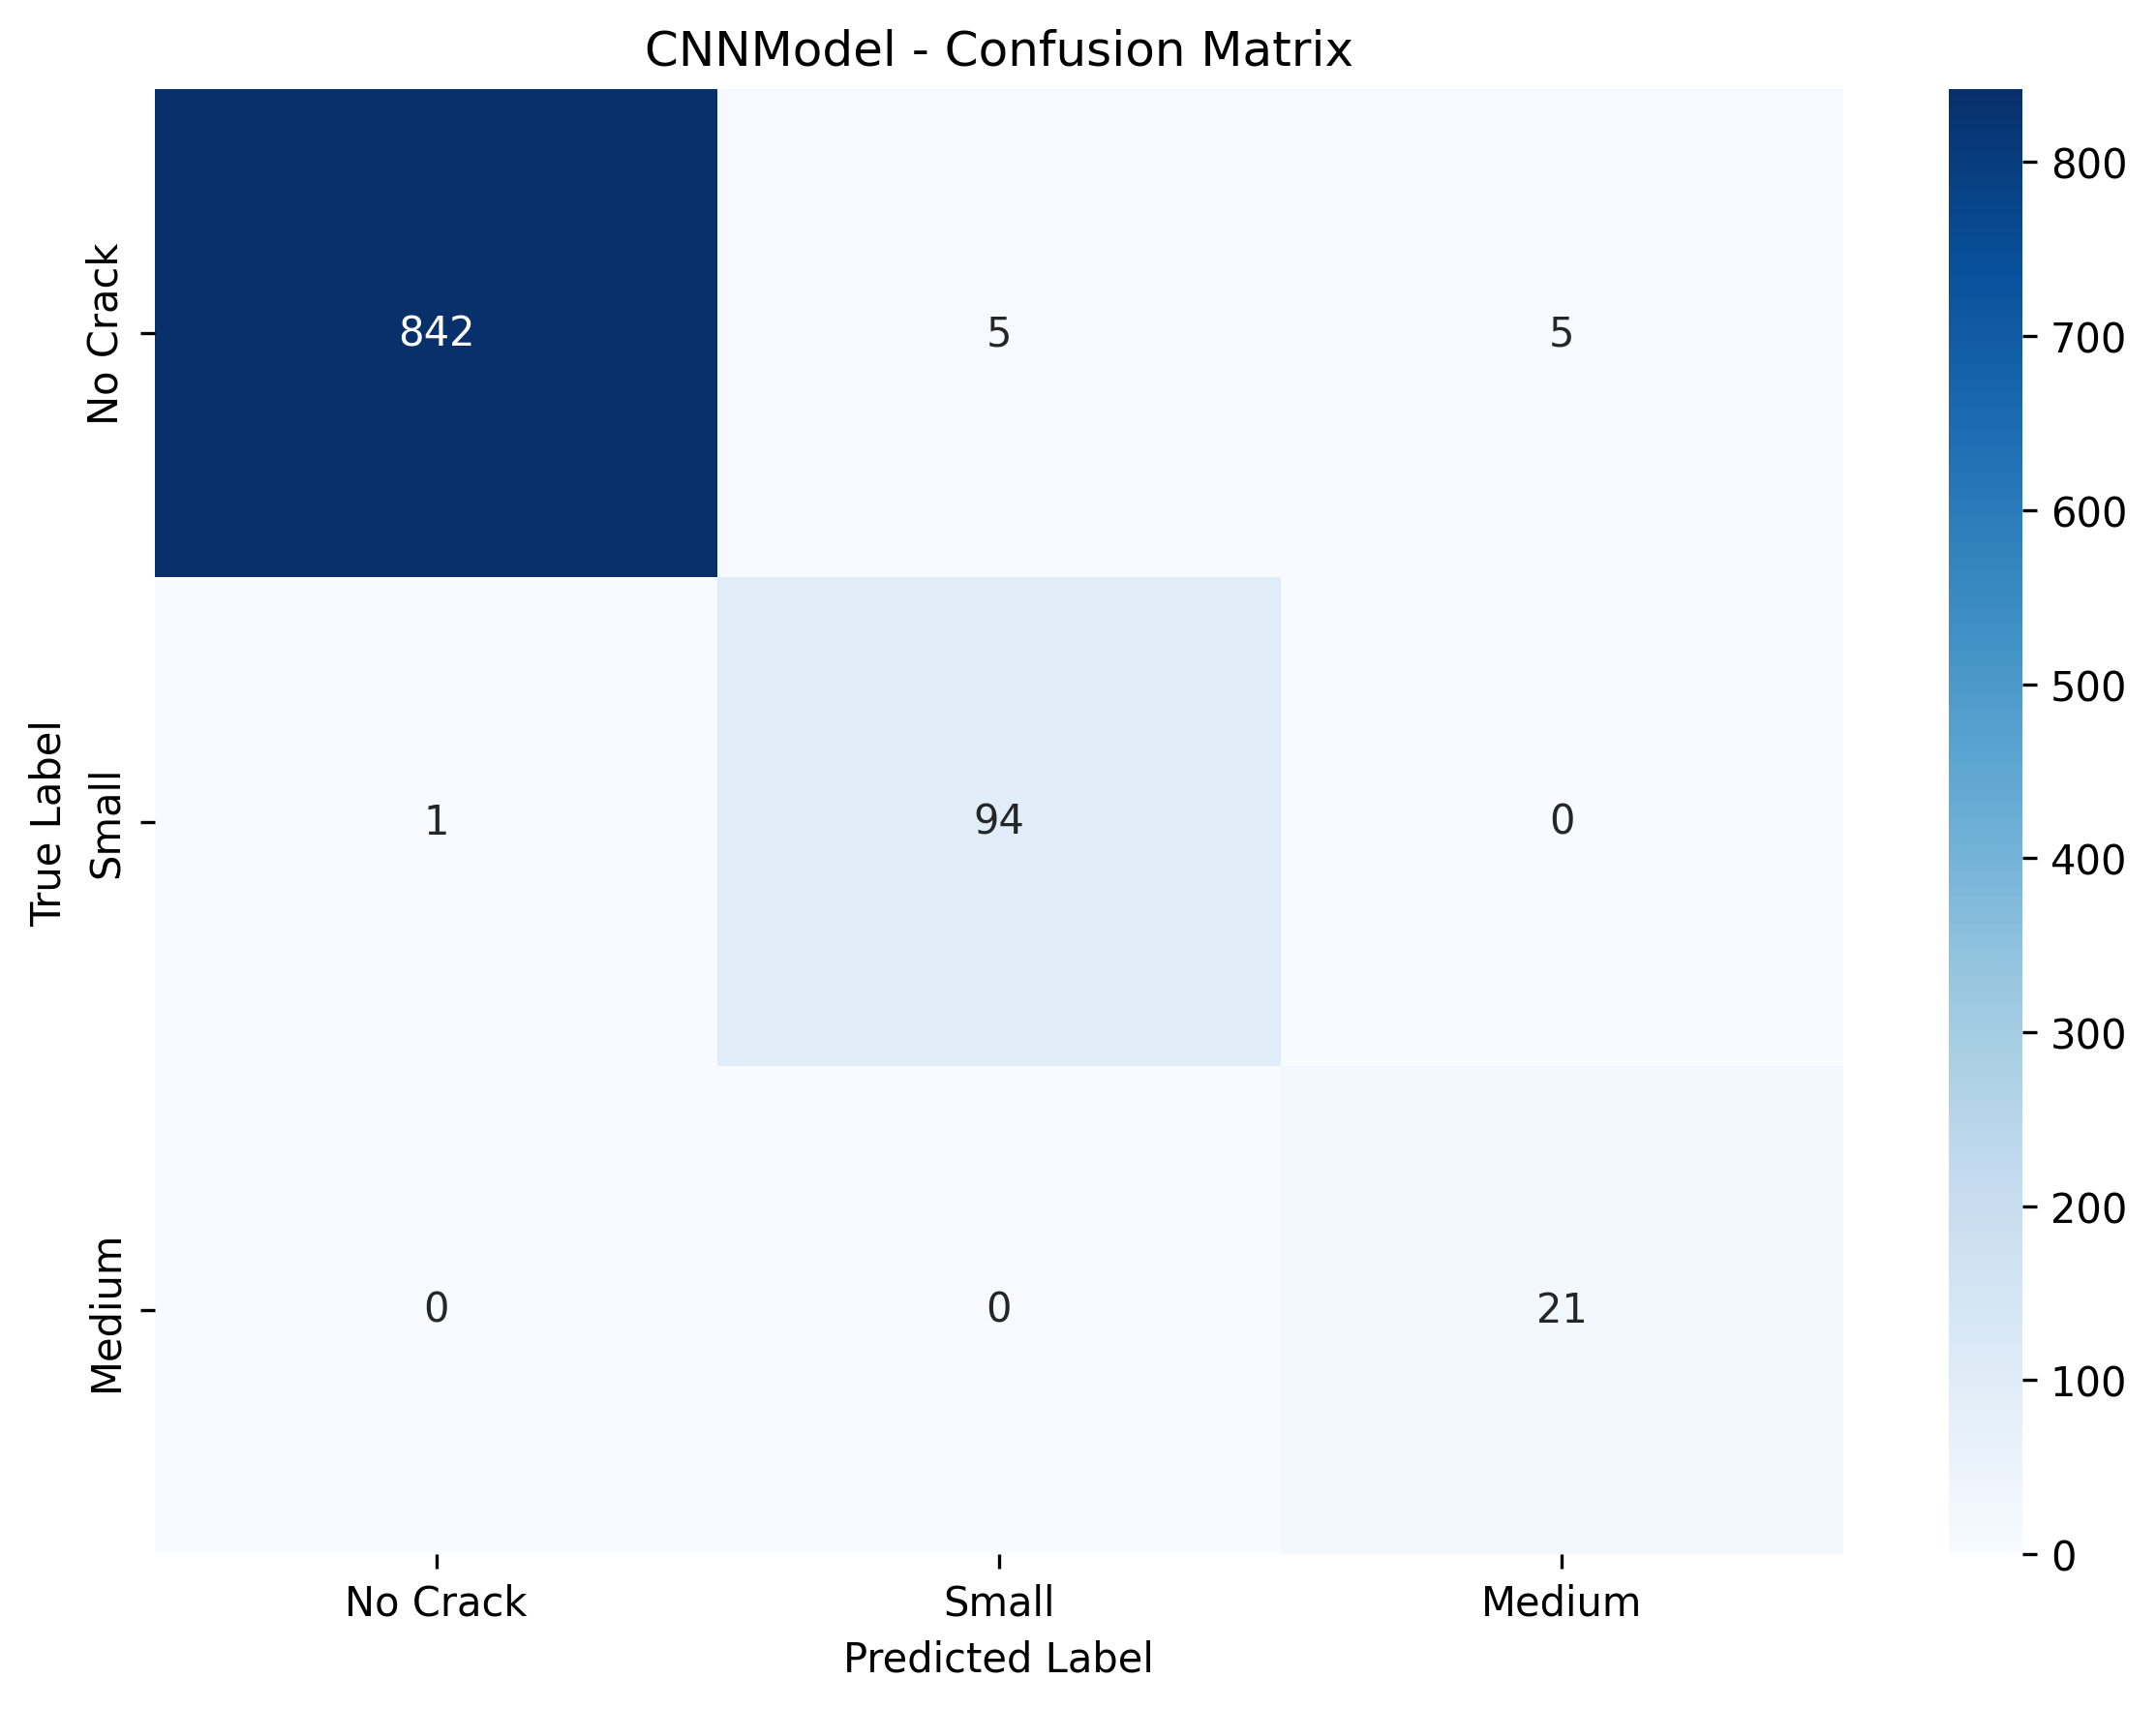
\includegraphics[width=0.7\textwidth]{img/CNNModel_confusion_matrix_100pct.png}
    \caption{Confusion Matrix for the CNN Model.}
    \label{fig:cnn_cm}
\end{figure}

\subsection{Impact of Training Data Size on CNN Performance}
To investigate the effect of training data volume on the CNN model's performance, an experiment was conducted where the model was trained on varying percentages of the training dataset. The training size was incrementally increased from 5\% to 100\% with a step size of 5\%.

The results, shown in Figure \ref{fig:training_percentage}, demonstrate that the model's accuracy improves significantly with more data, as expected. However, it reaches a peak accuracy of 99.0\% with only 65\% and 70\% of the training data. This suggests that the model can achieve optimal performance without requiring the entire dataset, potentially reducing training time and computational resources. The confusion matrix for the model trained on 65\% of the data, shown in Figure \ref{fig:cnn_cm_65pct}, confirms this high level of performance.

\begin{figure}[H]
    \centering
    \includegraphics[width=0.8\textwidth]{img/training_percentage_analysis.png}
    \caption{Test Accuracy vs. Training Data Percentage for the CNN Model.}
    \label{fig:training_percentage}
\end{figure}

\begin{figure}[H]
    \centering
    
\includegraphics[width=0.7\textwidth]{img/CNNModel_confusion_matrix_65pct.png}
    \caption{Confusion Matrix for the CNN Model Trained on 65\% of the Data.}
    \label{fig:cnn_cm_65pct}
\end{figure}

\subsection{Model Comparison}
Both the Random Forest and the CNN models showed excellent performance. However, it is worth noting the different strengths of each approach, especially concerning the imbalanced nature of the dataset.

A Random Forest is an ensemble model, which means it builds random decision trees on different sub-samples of the data. This structure makes it inherently robust against overfitting and effective at handling imbalanced classes. Even if individual trees are biased towards the majority class, the ensemble as a whole can still learn the patterns of the minority classes effectively. For a more detailed visual explanation of the Random Forest algorithm, please refer to the supplementary document in Teams Channel of ours: \texttt{Explanation\_of\_Random\_Forest.pdf}.

The CNN, on the other hand, is designed to learn hierarchical patterns directly from sequence data. While powerful, it can be more sensitive to class imbalance. In this project, this was mitigated by applying class weights to the loss function, which penalizes the model more for misclassifying the minority classes. Despite this, for datasets with a limited number of samples for the minority classes, a Random Forest can provide a more stable and reliable performance with less tuning required.

\end{document}
